% Created by tikzDevice version 0.12.6 on 2026-03-06 18:19:36
% !TEX encoding = UTF-8 Unicode
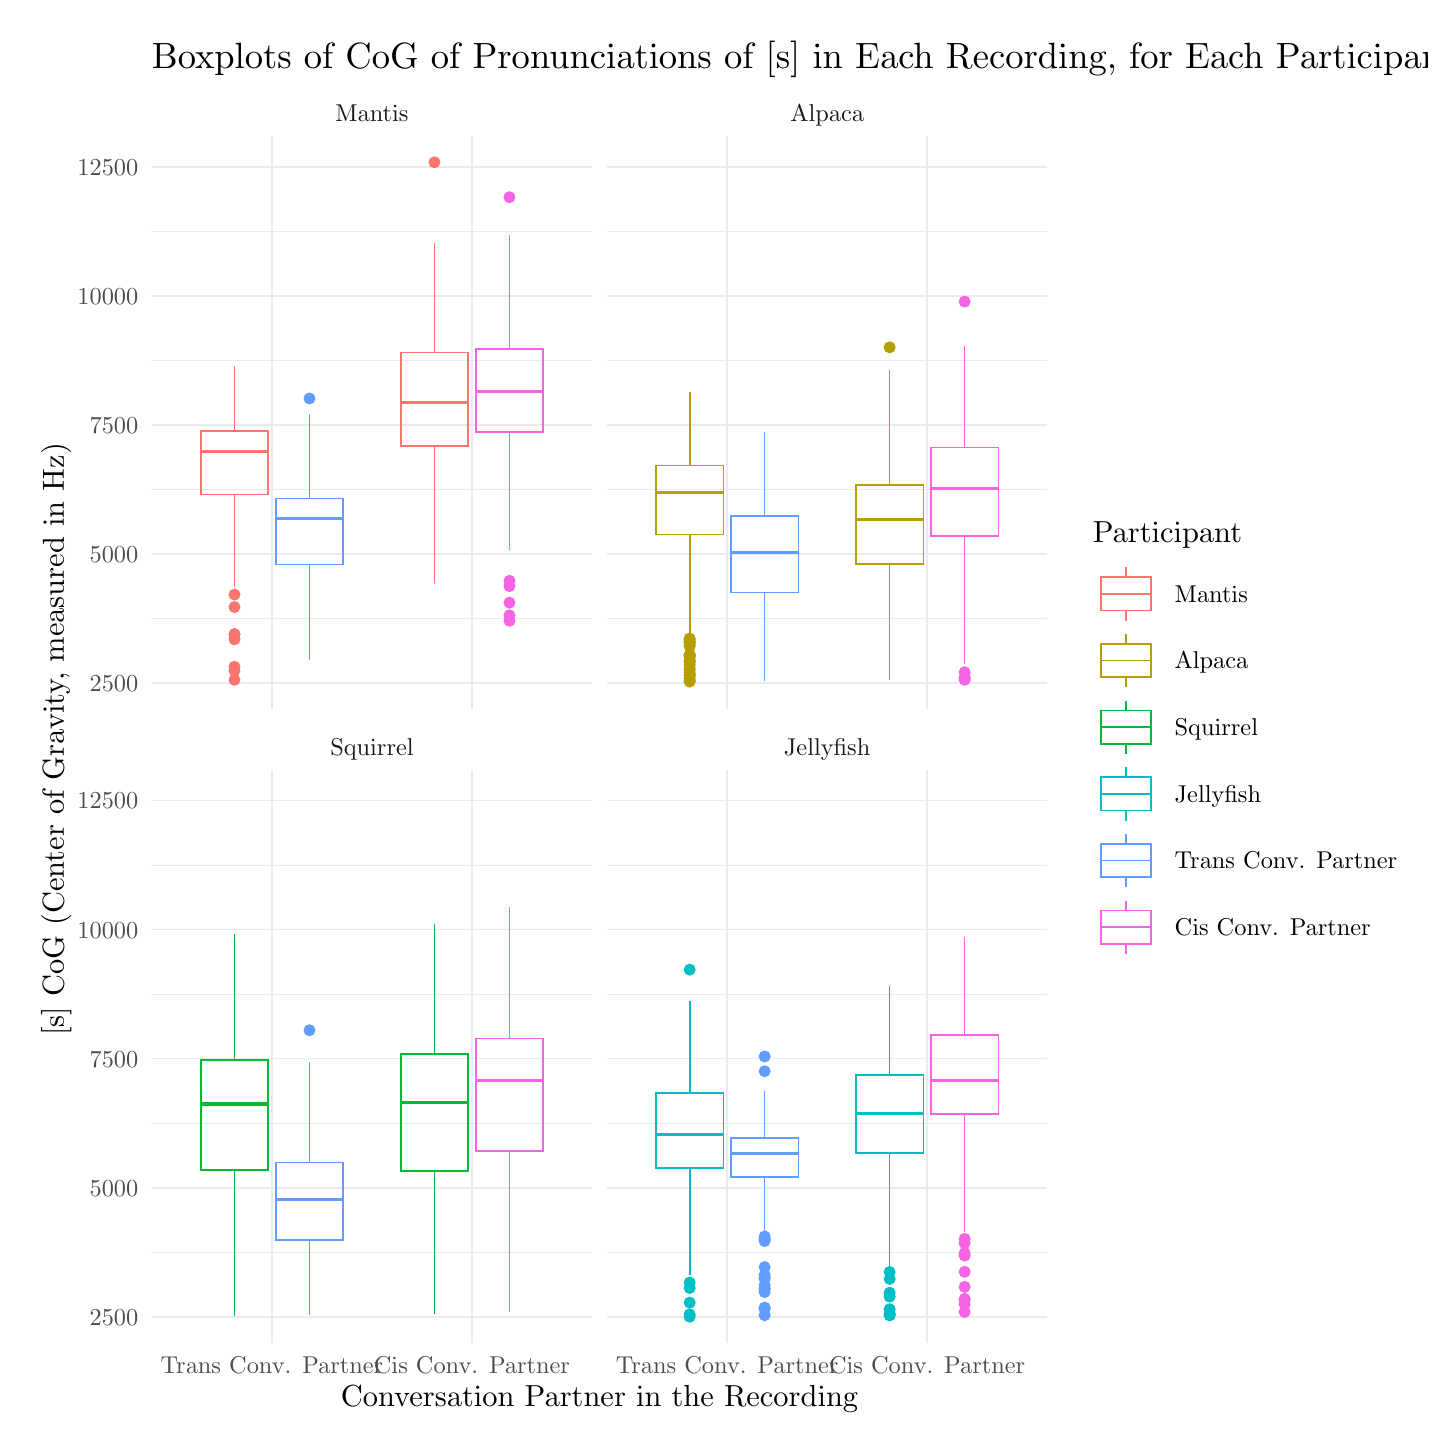
\begin{tikzpicture}[x=1pt,y=1pt]
\definecolor{fillColor}{RGB}{255,255,255}
\path[use as bounding box,fill=fillColor,fill opacity=0.00] (0,0) rectangle (505.89,505.89);
\begin{scope}
\path[clip] (  0.00,  0.00) rectangle (505.89,505.89);
\definecolor{fillColor}{RGB}{255,255,255}

\path[fill=fillColor] (  0.00,  0.00) rectangle (505.89,505.89);
\end{scope}
\begin{scope}
\path[clip] ( 44.92,259.71) rectangle (203.90,466.66);
\definecolor{drawColor}{gray}{0.92}

\path[draw=drawColor,line width= 0.3pt,line join=round] ( 44.92,292.41) --
	(203.90,292.41);

\path[draw=drawColor,line width= 0.3pt,line join=round] ( 44.92,339.04) --
	(203.90,339.04);

\path[draw=drawColor,line width= 0.3pt,line join=round] ( 44.92,385.67) --
	(203.90,385.67);

\path[draw=drawColor,line width= 0.3pt,line join=round] ( 44.92,432.30) --
	(203.90,432.30);

\path[draw=drawColor,line width= 0.6pt,line join=round] ( 44.92,269.10) --
	(203.90,269.10);

\path[draw=drawColor,line width= 0.6pt,line join=round] ( 44.92,315.73) --
	(203.90,315.73);

\path[draw=drawColor,line width= 0.6pt,line join=round] ( 44.92,362.36) --
	(203.90,362.36);

\path[draw=drawColor,line width= 0.6pt,line join=round] ( 44.92,408.98) --
	(203.90,408.98);

\path[draw=drawColor,line width= 0.6pt,line join=round] ( 44.92,455.61) --
	(203.90,455.61);

\path[draw=drawColor,line width= 0.6pt,line join=round] ( 88.27,259.71) --
	( 88.27,466.66);

\path[draw=drawColor,line width= 0.6pt,line join=round] (160.54,259.71) --
	(160.54,466.66);
\end{scope}
\begin{scope}
\path[clip] ( 44.92,259.71) rectangle (203.90,466.66);
\definecolor{drawColor}{RGB}{248,118,109}
\definecolor{fillColor}{RGB}{248,118,109}

\path[draw=drawColor,line width= 0.4pt,line join=round,line cap=round,fill=fillColor] ( 74.73,286.68) circle (  1.96);

\path[draw=drawColor,line width= 0.4pt,line join=round,line cap=round,fill=fillColor] ( 74.73,274.94) circle (  1.96);

\path[draw=drawColor,line width= 0.4pt,line join=round,line cap=round,fill=fillColor] ( 74.73,296.53) circle (  1.96);

\path[draw=drawColor,line width= 0.4pt,line join=round,line cap=round,fill=fillColor] ( 74.73,270.24) circle (  1.96);

\path[draw=drawColor,line width= 0.4pt,line join=round,line cap=round,fill=fillColor] ( 74.73,273.59) circle (  1.96);

\path[draw=drawColor,line width= 0.4pt,line join=round,line cap=round,fill=fillColor] ( 74.73,286.75) circle (  1.96);

\path[draw=drawColor,line width= 0.4pt,line join=round,line cap=round,fill=fillColor] ( 74.73,301.04) circle (  1.96);

\path[draw=drawColor,line width= 0.4pt,line join=round,line cap=round,fill=fillColor] ( 74.73,284.89) circle (  1.96);

\path[draw=drawColor,line width= 0.6pt,line join=round] ( 74.73,360.23) -- ( 74.73,383.68);

\path[draw=drawColor,line width= 0.6pt,line join=round] ( 74.73,337.18) -- ( 74.73,303.60);
\end{scope}
\begin{scope}
\path[clip] ( 44.92,259.71) rectangle (203.90,466.66);
\definecolor{drawColor}{RGB}{248,118,109}

\path[draw=drawColor,line width= 0.6pt] ( 62.53,360.23) --
	( 62.53,337.18) --
	( 86.92,337.18) --
	( 86.92,360.23) --
	( 62.53,360.23) --
	cycle;

\path[draw=drawColor,line width= 1.1pt] ( 62.53,352.64) -- ( 86.92,352.64);
\end{scope}
\begin{scope}
\path[clip] ( 44.92,259.71) rectangle (203.90,466.66);
\definecolor{drawColor}{RGB}{97,156,255}
\definecolor{fillColor}{RGB}{97,156,255}

\path[draw=drawColor,line width= 0.4pt,line join=round,line cap=round,fill=fillColor] (101.82,371.90) circle (  1.96);

\path[draw=drawColor,line width= 0.6pt,line join=round] (101.82,335.76) -- (101.82,366.44);

\path[draw=drawColor,line width= 0.6pt,line join=round] (101.82,311.91) -- (101.82,277.41);
\end{scope}
\begin{scope}
\path[clip] ( 44.92,259.71) rectangle (203.90,466.66);
\definecolor{drawColor}{RGB}{97,156,255}

\path[draw=drawColor,line width= 0.6pt] ( 89.63,335.76) --
	( 89.63,311.91) --
	(114.02,311.91) --
	(114.02,335.76) --
	( 89.63,335.76) --
	cycle;

\path[draw=drawColor,line width= 1.1pt] ( 89.63,328.52) -- (114.02,328.52);
\end{scope}
\begin{scope}
\path[clip] ( 44.92,259.71) rectangle (203.90,466.66);
\definecolor{drawColor}{RGB}{248,118,109}
\definecolor{fillColor}{RGB}{248,118,109}

\path[draw=drawColor,line width= 0.4pt,line join=round,line cap=round,fill=fillColor] (146.99,457.25) circle (  1.96);

\path[draw=drawColor,line width= 0.6pt,line join=round] (146.99,388.48) -- (146.99,427.98);

\path[draw=drawColor,line width= 0.6pt,line join=round] (146.99,354.70) -- (146.99,305.31);
\end{scope}
\begin{scope}
\path[clip] ( 44.92,259.71) rectangle (203.90,466.66);
\definecolor{drawColor}{RGB}{248,118,109}

\path[draw=drawColor,line width= 0.6pt] (134.79,388.48) --
	(134.79,354.70) --
	(159.18,354.70) --
	(159.18,388.48) --
	(134.79,388.48) --
	cycle;

\path[draw=drawColor,line width= 1.1pt] (134.79,370.53) -- (159.18,370.53);
\end{scope}
\begin{scope}
\path[clip] ( 44.92,259.71) rectangle (203.90,466.66);
\definecolor{drawColor}{RGB}{245,100,227}
\definecolor{fillColor}{RGB}{245,100,227}

\path[draw=drawColor,line width= 0.4pt,line join=round,line cap=round,fill=fillColor] (174.09,293.53) circle (  1.96);

\path[draw=drawColor,line width= 0.4pt,line join=round,line cap=round,fill=fillColor] (174.09,444.63) circle (  1.96);

\path[draw=drawColor,line width= 0.4pt,line join=round,line cap=round,fill=fillColor] (174.09,298.11) circle (  1.96);

\path[draw=drawColor,line width= 0.4pt,line join=round,line cap=round,fill=fillColor] (174.09,304.10) circle (  1.96);

\path[draw=drawColor,line width= 0.4pt,line join=round,line cap=round,fill=fillColor] (174.09,291.59) circle (  1.96);

\path[draw=drawColor,line width= 0.4pt,line join=round,line cap=round,fill=fillColor] (174.09,306.01) circle (  1.96);

\path[draw=drawColor,line width= 0.6pt,line join=round] (174.09,389.69) -- (174.09,430.82);

\path[draw=drawColor,line width= 0.6pt,line join=round] (174.09,359.73) -- (174.09,317.20);
\end{scope}
\begin{scope}
\path[clip] ( 44.92,259.71) rectangle (203.90,466.66);
\definecolor{drawColor}{RGB}{245,100,227}

\path[draw=drawColor,line width= 0.6pt] (161.89,389.69) --
	(161.89,359.73) --
	(186.28,359.73) --
	(186.28,389.69) --
	(161.89,389.69) --
	cycle;

\path[draw=drawColor,line width= 1.1pt] (161.89,374.51) -- (186.28,374.51);
\end{scope}
\begin{scope}
\path[clip] ( 44.92, 30.69) rectangle (203.90,237.64);
\definecolor{drawColor}{gray}{0.92}

\path[draw=drawColor,line width= 0.3pt,line join=round] ( 44.92, 63.39) --
	(203.90, 63.39);

\path[draw=drawColor,line width= 0.3pt,line join=round] ( 44.92,110.02) --
	(203.90,110.02);

\path[draw=drawColor,line width= 0.3pt,line join=round] ( 44.92,156.65) --
	(203.90,156.65);

\path[draw=drawColor,line width= 0.3pt,line join=round] ( 44.92,203.28) --
	(203.90,203.28);

\path[draw=drawColor,line width= 0.6pt,line join=round] ( 44.92, 40.08) --
	(203.90, 40.08);

\path[draw=drawColor,line width= 0.6pt,line join=round] ( 44.92, 86.71) --
	(203.90, 86.71);

\path[draw=drawColor,line width= 0.6pt,line join=round] ( 44.92,133.34) --
	(203.90,133.34);

\path[draw=drawColor,line width= 0.6pt,line join=round] ( 44.92,179.96) --
	(203.90,179.96);

\path[draw=drawColor,line width= 0.6pt,line join=round] ( 44.92,226.59) --
	(203.90,226.59);

\path[draw=drawColor,line width= 0.6pt,line join=round] ( 88.27, 30.69) --
	( 88.27,237.64);

\path[draw=drawColor,line width= 0.6pt,line join=round] (160.54, 30.69) --
	(160.54,237.64);
\definecolor{drawColor}{RGB}{0,186,56}

\path[draw=drawColor,line width= 0.6pt,line join=round] ( 74.73,132.84) -- ( 74.73,178.46);

\path[draw=drawColor,line width= 0.6pt,line join=round] ( 74.73, 93.21) -- ( 74.73, 40.28);
\end{scope}
\begin{scope}
\path[clip] ( 44.92, 30.69) rectangle (203.90,237.64);
\definecolor{drawColor}{RGB}{0,186,56}

\path[draw=drawColor,line width= 0.6pt] ( 62.53,132.84) --
	( 62.53, 93.21) --
	( 86.92, 93.21) --
	( 86.92,132.84) --
	( 62.53,132.84) --
	cycle;

\path[draw=drawColor,line width= 1.1pt] ( 62.53,116.96) -- ( 86.92,116.96);
\end{scope}
\begin{scope}
\path[clip] ( 44.92, 30.69) rectangle (203.90,237.64);
\definecolor{drawColor}{RGB}{97,156,255}
\definecolor{fillColor}{RGB}{97,156,255}

\path[draw=drawColor,line width= 0.4pt,line join=round,line cap=round,fill=fillColor] (101.82,143.61) circle (  1.96);

\path[draw=drawColor,line width= 0.6pt,line join=round] (101.82, 95.77) -- (101.82,132.10);

\path[draw=drawColor,line width= 0.6pt,line join=round] (101.82, 67.81) -- (101.82, 40.70);
\end{scope}
\begin{scope}
\path[clip] ( 44.92, 30.69) rectangle (203.90,237.64);
\definecolor{drawColor}{RGB}{97,156,255}

\path[draw=drawColor,line width= 0.6pt] ( 89.63, 95.77) --
	( 89.63, 67.81) --
	(114.02, 67.81) --
	(114.02, 95.77) --
	( 89.63, 95.77) --
	cycle;

\path[draw=drawColor,line width= 1.1pt] ( 89.63, 82.56) -- (114.02, 82.56);
\definecolor{drawColor}{RGB}{0,186,56}

\path[draw=drawColor,line width= 0.6pt,line join=round] (146.99,135.04) -- (146.99,182.02);

\path[draw=drawColor,line width= 0.6pt,line join=round] (146.99, 92.85) -- (146.99, 41.02);
\end{scope}
\begin{scope}
\path[clip] ( 44.92, 30.69) rectangle (203.90,237.64);
\definecolor{drawColor}{RGB}{0,186,56}

\path[draw=drawColor,line width= 0.6pt] (134.79,135.04) --
	(134.79, 92.85) --
	(159.18, 92.85) --
	(159.18,135.04) --
	(134.79,135.04) --
	cycle;

\path[draw=drawColor,line width= 1.1pt] (134.79,117.39) -- (159.18,117.39);
\definecolor{drawColor}{RGB}{245,100,227}

\path[draw=drawColor,line width= 0.6pt,line join=round] (174.09,140.66) -- (174.09,188.17);

\path[draw=drawColor,line width= 0.6pt,line join=round] (174.09, 99.99) -- (174.09, 41.96);
\end{scope}
\begin{scope}
\path[clip] ( 44.92, 30.69) rectangle (203.90,237.64);
\definecolor{drawColor}{RGB}{245,100,227}

\path[draw=drawColor,line width= 0.6pt] (161.89,140.66) --
	(161.89, 99.99) --
	(186.28, 99.99) --
	(186.28,140.66) --
	(161.89,140.66) --
	cycle;

\path[draw=drawColor,line width= 1.1pt] (161.89,125.61) -- (186.28,125.61);
\end{scope}
\begin{scope}
\path[clip] (209.40,259.71) rectangle (368.38,466.66);
\definecolor{drawColor}{gray}{0.92}

\path[draw=drawColor,line width= 0.3pt,line join=round] (209.40,292.41) --
	(368.38,292.41);

\path[draw=drawColor,line width= 0.3pt,line join=round] (209.40,339.04) --
	(368.38,339.04);

\path[draw=drawColor,line width= 0.3pt,line join=round] (209.40,385.67) --
	(368.38,385.67);

\path[draw=drawColor,line width= 0.3pt,line join=round] (209.40,432.30) --
	(368.38,432.30);

\path[draw=drawColor,line width= 0.6pt,line join=round] (209.40,269.10) --
	(368.38,269.10);

\path[draw=drawColor,line width= 0.6pt,line join=round] (209.40,315.73) --
	(368.38,315.73);

\path[draw=drawColor,line width= 0.6pt,line join=round] (209.40,362.36) --
	(368.38,362.36);

\path[draw=drawColor,line width= 0.6pt,line join=round] (209.40,408.98) --
	(368.38,408.98);

\path[draw=drawColor,line width= 0.6pt,line join=round] (209.40,455.61) --
	(368.38,455.61);

\path[draw=drawColor,line width= 0.6pt,line join=round] (252.76,259.71) --
	(252.76,466.66);

\path[draw=drawColor,line width= 0.6pt,line join=round] (325.02,259.71) --
	(325.02,466.66);
\end{scope}
\begin{scope}
\path[clip] (209.40,259.71) rectangle (368.38,466.66);
\definecolor{drawColor}{RGB}{183,159,0}
\definecolor{fillColor}{RGB}{183,159,0}

\path[draw=drawColor,line width= 0.4pt,line join=round,line cap=round,fill=fillColor] (239.21,283.08) circle (  1.96);

\path[draw=drawColor,line width= 0.4pt,line join=round,line cap=round,fill=fillColor] (239.21,269.60) circle (  1.96);

\path[draw=drawColor,line width= 0.4pt,line join=round,line cap=round,fill=fillColor] (239.21,276.69) circle (  1.96);

\path[draw=drawColor,line width= 0.4pt,line join=round,line cap=round,fill=fillColor] (239.21,278.85) circle (  1.96);

\path[draw=drawColor,line width= 0.4pt,line join=round,line cap=round,fill=fillColor] (239.21,284.01) circle (  1.96);

\path[draw=drawColor,line width= 0.4pt,line join=round,line cap=round,fill=fillColor] (239.21,269.99) circle (  1.96);

\path[draw=drawColor,line width= 0.4pt,line join=round,line cap=round,fill=fillColor] (239.21,270.68) circle (  1.96);

\path[draw=drawColor,line width= 0.4pt,line join=round,line cap=round,fill=fillColor] (239.21,271.77) circle (  1.96);

\path[draw=drawColor,line width= 0.4pt,line join=round,line cap=round,fill=fillColor] (239.21,283.91) circle (  1.96);

\path[draw=drawColor,line width= 0.4pt,line join=round,line cap=round,fill=fillColor] (239.21,272.08) circle (  1.96);

\path[draw=drawColor,line width= 0.4pt,line join=round,line cap=round,fill=fillColor] (239.21,274.49) circle (  1.96);

\path[draw=drawColor,line width= 0.4pt,line join=round,line cap=round,fill=fillColor] (239.21,272.84) circle (  1.96);

\path[draw=drawColor,line width= 0.4pt,line join=round,line cap=round,fill=fillColor] (239.21,284.77) circle (  1.96);

\path[draw=drawColor,line width= 0.4pt,line join=round,line cap=round,fill=fillColor] (239.21,273.69) circle (  1.96);

\path[draw=drawColor,line width= 0.4pt,line join=round,line cap=round,fill=fillColor] (239.21,279.23) circle (  1.96);

\path[draw=drawColor,line width= 0.4pt,line join=round,line cap=round,fill=fillColor] (239.21,279.18) circle (  1.96);

\path[draw=drawColor,line width= 0.4pt,line join=round,line cap=round,fill=fillColor] (239.21,275.71) circle (  1.96);

\path[draw=drawColor,line width= 0.4pt,line join=round,line cap=round,fill=fillColor] (239.21,271.67) circle (  1.96);

\path[draw=drawColor,line width= 0.4pt,line join=round,line cap=round,fill=fillColor] (239.21,279.31) circle (  1.96);

\path[draw=drawColor,line width= 0.4pt,line join=round,line cap=round,fill=fillColor] (239.21,285.14) circle (  1.96);

\path[draw=drawColor,line width= 0.4pt,line join=round,line cap=round,fill=fillColor] (239.21,276.99) circle (  1.96);

\path[draw=drawColor,line width= 0.4pt,line join=round,line cap=round,fill=fillColor] (239.21,278.25) circle (  1.96);

\path[draw=drawColor,line width= 0.4pt,line join=round,line cap=round,fill=fillColor] (239.21,283.69) circle (  1.96);

\path[draw=drawColor,line width= 0.4pt,line join=round,line cap=round,fill=fillColor] (239.21,282.35) circle (  1.96);

\path[draw=drawColor,line width= 0.4pt,line join=round,line cap=round,fill=fillColor] (239.21,277.20) circle (  1.96);

\path[draw=drawColor,line width= 0.6pt,line join=round] (239.21,347.69) -- (239.21,374.25);

\path[draw=drawColor,line width= 0.6pt,line join=round] (239.21,322.71) -- (239.21,285.37);
\end{scope}
\begin{scope}
\path[clip] (209.40,259.71) rectangle (368.38,466.66);
\definecolor{drawColor}{RGB}{183,159,0}

\path[draw=drawColor,line width= 0.6pt] (227.01,347.69) --
	(227.01,322.71) --
	(251.40,322.71) --
	(251.40,347.69) --
	(227.01,347.69) --
	cycle;

\path[draw=drawColor,line width= 1.1pt] (227.01,337.91) -- (251.40,337.91);
\definecolor{drawColor}{RGB}{97,156,255}

\path[draw=drawColor,line width= 0.6pt,line join=round] (266.30,329.31) -- (266.30,359.77);

\path[draw=drawColor,line width= 0.6pt,line join=round] (266.30,301.74) -- (266.30,269.66);
\end{scope}
\begin{scope}
\path[clip] (209.40,259.71) rectangle (368.38,466.66);
\definecolor{drawColor}{RGB}{97,156,255}

\path[draw=drawColor,line width= 0.6pt] (254.11,329.31) --
	(254.11,301.74) --
	(278.50,301.74) --
	(278.50,329.31) --
	(254.11,329.31) --
	cycle;

\path[draw=drawColor,line width= 1.1pt] (254.11,316.33) -- (278.50,316.33);
\end{scope}
\begin{scope}
\path[clip] (209.40,259.71) rectangle (368.38,466.66);
\definecolor{drawColor}{RGB}{183,159,0}
\definecolor{fillColor}{RGB}{183,159,0}

\path[draw=drawColor,line width= 0.4pt,line join=round,line cap=round,fill=fillColor] (311.47,390.38) circle (  1.96);

\path[draw=drawColor,line width= 0.6pt,line join=round] (311.47,340.53) -- (311.47,382.16);

\path[draw=drawColor,line width= 0.6pt,line join=round] (311.47,312.11) -- (311.47,270.02);
\end{scope}
\begin{scope}
\path[clip] (209.40,259.71) rectangle (368.38,466.66);
\definecolor{drawColor}{RGB}{183,159,0}

\path[draw=drawColor,line width= 0.6pt] (299.28,340.53) --
	(299.28,312.11) --
	(323.66,312.11) --
	(323.66,340.53) --
	(299.28,340.53) --
	cycle;

\path[draw=drawColor,line width= 1.1pt] (299.28,328.33) -- (323.66,328.33);
\end{scope}
\begin{scope}
\path[clip] (209.40,259.71) rectangle (368.38,466.66);
\definecolor{drawColor}{RGB}{245,100,227}
\definecolor{fillColor}{RGB}{245,100,227}

\path[draw=drawColor,line width= 0.4pt,line join=round,line cap=round,fill=fillColor] (338.57,270.92) circle (  1.96);

\path[draw=drawColor,line width= 0.4pt,line join=round,line cap=round,fill=fillColor] (338.57,270.25) circle (  1.96);

\path[draw=drawColor,line width= 0.4pt,line join=round,line cap=round,fill=fillColor] (338.57,271.16) circle (  1.96);

\path[draw=drawColor,line width= 0.4pt,line join=round,line cap=round,fill=fillColor] (338.57,406.90) circle (  1.96);

\path[draw=drawColor,line width= 0.4pt,line join=round,line cap=round,fill=fillColor] (338.57,272.97) circle (  1.96);

\path[draw=drawColor,line width= 0.6pt,line join=round] (338.57,354.19) -- (338.57,390.82);

\path[draw=drawColor,line width= 0.6pt,line join=round] (338.57,322.28) -- (338.57,276.00);
\end{scope}
\begin{scope}
\path[clip] (209.40,259.71) rectangle (368.38,466.66);
\definecolor{drawColor}{RGB}{245,100,227}

\path[draw=drawColor,line width= 0.6pt] (326.37,354.19) --
	(326.37,322.28) --
	(350.76,322.28) --
	(350.76,354.19) --
	(326.37,354.19) --
	cycle;

\path[draw=drawColor,line width= 1.1pt] (326.37,339.52) -- (350.76,339.52);
\end{scope}
\begin{scope}
\path[clip] (209.40, 30.69) rectangle (368.38,237.64);
\definecolor{drawColor}{gray}{0.92}

\path[draw=drawColor,line width= 0.3pt,line join=round] (209.40, 63.39) --
	(368.38, 63.39);

\path[draw=drawColor,line width= 0.3pt,line join=round] (209.40,110.02) --
	(368.38,110.02);

\path[draw=drawColor,line width= 0.3pt,line join=round] (209.40,156.65) --
	(368.38,156.65);

\path[draw=drawColor,line width= 0.3pt,line join=round] (209.40,203.28) --
	(368.38,203.28);

\path[draw=drawColor,line width= 0.6pt,line join=round] (209.40, 40.08) --
	(368.38, 40.08);

\path[draw=drawColor,line width= 0.6pt,line join=round] (209.40, 86.71) --
	(368.38, 86.71);

\path[draw=drawColor,line width= 0.6pt,line join=round] (209.40,133.34) --
	(368.38,133.34);

\path[draw=drawColor,line width= 0.6pt,line join=round] (209.40,179.96) --
	(368.38,179.96);

\path[draw=drawColor,line width= 0.6pt,line join=round] (209.40,226.59) --
	(368.38,226.59);

\path[draw=drawColor,line width= 0.6pt,line join=round] (252.76, 30.69) --
	(252.76,237.64);

\path[draw=drawColor,line width= 0.6pt,line join=round] (325.02, 30.69) --
	(325.02,237.64);
\end{scope}
\begin{scope}
\path[clip] (209.40, 30.69) rectangle (368.38,237.64);
\definecolor{drawColor}{RGB}{0,191,196}
\definecolor{fillColor}{RGB}{0,191,196}

\path[draw=drawColor,line width= 0.4pt,line join=round,line cap=round,fill=fillColor] (239.21, 52.45) circle (  1.96);

\path[draw=drawColor,line width= 0.4pt,line join=round,line cap=round,fill=fillColor] (239.21, 45.19) circle (  1.96);

\path[draw=drawColor,line width= 0.4pt,line join=round,line cap=round,fill=fillColor] (239.21, 40.10) circle (  1.96);

\path[draw=drawColor,line width= 0.4pt,line join=round,line cap=round,fill=fillColor] (239.21, 50.46) circle (  1.96);

\path[draw=drawColor,line width= 0.4pt,line join=round,line cap=round,fill=fillColor] (239.21, 40.97) circle (  1.96);

\path[draw=drawColor,line width= 0.4pt,line join=round,line cap=round,fill=fillColor] (239.21,165.50) circle (  1.96);

\path[draw=drawColor,line width= 0.6pt,line join=round] (239.21,120.85) -- (239.21,154.27);

\path[draw=drawColor,line width= 0.6pt,line join=round] (239.21, 93.73) -- (239.21, 55.13);
\end{scope}
\begin{scope}
\path[clip] (209.40, 30.69) rectangle (368.38,237.64);
\definecolor{drawColor}{RGB}{0,191,196}

\path[draw=drawColor,line width= 0.6pt] (227.01,120.85) --
	(227.01, 93.73) --
	(251.40, 93.73) --
	(251.40,120.85) --
	(227.01,120.85) --
	cycle;

\path[draw=drawColor,line width= 1.1pt] (227.01,105.95) -- (251.40,105.95);
\end{scope}
\begin{scope}
\path[clip] (209.40, 30.69) rectangle (368.38,237.64);
\definecolor{drawColor}{RGB}{97,156,255}
\definecolor{fillColor}{RGB}{97,156,255}

\path[draw=drawColor,line width= 0.4pt,line join=round,line cap=round,fill=fillColor] (266.30, 43.15) circle (  1.96);

\path[draw=drawColor,line width= 0.4pt,line join=round,line cap=round,fill=fillColor] (266.30, 68.25) circle (  1.96);

\path[draw=drawColor,line width= 0.4pt,line join=round,line cap=round,fill=fillColor] (266.30, 69.08) circle (  1.96);

\path[draw=drawColor,line width= 0.4pt,line join=round,line cap=round,fill=fillColor] (266.30,134.13) circle (  1.96);

\path[draw=drawColor,line width= 0.4pt,line join=round,line cap=round,fill=fillColor] (266.30, 50.25) circle (  1.96);

\path[draw=drawColor,line width= 0.4pt,line join=round,line cap=round,fill=fillColor] (266.30, 67.94) circle (  1.96);

\path[draw=drawColor,line width= 0.4pt,line join=round,line cap=round,fill=fillColor] (266.30, 53.78) circle (  1.96);

\path[draw=drawColor,line width= 0.4pt,line join=round,line cap=round,fill=fillColor] (266.30, 50.13) circle (  1.96);

\path[draw=drawColor,line width= 0.4pt,line join=round,line cap=round,fill=fillColor] (266.30, 67.43) circle (  1.96);

\path[draw=drawColor,line width= 0.4pt,line join=round,line cap=round,fill=fillColor] (266.30, 40.66) circle (  1.96);

\path[draw=drawColor,line width= 0.4pt,line join=round,line cap=round,fill=fillColor] (266.30, 49.00) circle (  1.96);

\path[draw=drawColor,line width= 0.4pt,line join=round,line cap=round,fill=fillColor] (266.30, 51.52) circle (  1.96);

\path[draw=drawColor,line width= 0.4pt,line join=round,line cap=round,fill=fillColor] (266.30, 54.35) circle (  1.96);

\path[draw=drawColor,line width= 0.4pt,line join=round,line cap=round,fill=fillColor] (266.30, 55.20) circle (  1.96);

\path[draw=drawColor,line width= 0.4pt,line join=round,line cap=round,fill=fillColor] (266.30, 43.39) circle (  1.96);

\path[draw=drawColor,line width= 0.4pt,line join=round,line cap=round,fill=fillColor] (266.30, 58.03) circle (  1.96);

\path[draw=drawColor,line width= 0.4pt,line join=round,line cap=round,fill=fillColor] (266.30, 42.92) circle (  1.96);

\path[draw=drawColor,line width= 0.4pt,line join=round,line cap=round,fill=fillColor] (266.30,128.81) circle (  1.96);

\path[draw=drawColor,line width= 0.6pt,line join=round] (266.30,104.78) -- (266.30,121.81);

\path[draw=drawColor,line width= 0.6pt,line join=round] (266.30, 90.65) -- (266.30, 69.99);
\end{scope}
\begin{scope}
\path[clip] (209.40, 30.69) rectangle (368.38,237.64);
\definecolor{drawColor}{RGB}{97,156,255}

\path[draw=drawColor,line width= 0.6pt] (254.11,104.78) --
	(254.11, 90.65) --
	(278.50, 90.65) --
	(278.50,104.78) --
	(254.11,104.78) --
	cycle;

\path[draw=drawColor,line width= 1.1pt] (254.11, 99.11) -- (278.50, 99.11);
\end{scope}
\begin{scope}
\path[clip] (209.40, 30.69) rectangle (368.38,237.64);
\definecolor{drawColor}{RGB}{0,191,196}
\definecolor{fillColor}{RGB}{0,191,196}

\path[draw=drawColor,line width= 0.4pt,line join=round,line cap=round,fill=fillColor] (311.47, 56.25) circle (  1.96);

\path[draw=drawColor,line width= 0.4pt,line join=round,line cap=round,fill=fillColor] (311.47, 53.76) circle (  1.96);

\path[draw=drawColor,line width= 0.4pt,line join=round,line cap=round,fill=fillColor] (311.47, 42.81) circle (  1.96);

\path[draw=drawColor,line width= 0.4pt,line join=round,line cap=round,fill=fillColor] (311.47, 40.77) circle (  1.96);

\path[draw=drawColor,line width= 0.4pt,line join=round,line cap=round,fill=fillColor] (311.47, 48.77) circle (  1.96);

\path[draw=drawColor,line width= 0.4pt,line join=round,line cap=round,fill=fillColor] (311.47, 40.56) circle (  1.96);

\path[draw=drawColor,line width= 0.4pt,line join=round,line cap=round,fill=fillColor] (311.47, 41.20) circle (  1.96);

\path[draw=drawColor,line width= 0.4pt,line join=round,line cap=round,fill=fillColor] (311.47, 47.35) circle (  1.96);

\path[draw=drawColor,line width= 0.6pt,line join=round] (311.47,127.42) -- (311.47,159.51);

\path[draw=drawColor,line width= 0.6pt,line join=round] (311.47, 99.30) -- (311.47, 57.49);
\end{scope}
\begin{scope}
\path[clip] (209.40, 30.69) rectangle (368.38,237.64);
\definecolor{drawColor}{RGB}{0,191,196}

\path[draw=drawColor,line width= 0.6pt] (299.28,127.42) --
	(299.28, 99.30) --
	(323.66, 99.30) --
	(323.66,127.42) --
	(299.28,127.42) --
	cycle;

\path[draw=drawColor,line width= 1.1pt] (299.28,113.40) -- (323.66,113.40);
\end{scope}
\begin{scope}
\path[clip] (209.40, 30.69) rectangle (368.38,237.64);
\definecolor{drawColor}{RGB}{245,100,227}
\definecolor{fillColor}{RGB}{245,100,227}

\path[draw=drawColor,line width= 0.4pt,line join=round,line cap=round,fill=fillColor] (338.57, 56.31) circle (  1.96);

\path[draw=drawColor,line width= 0.4pt,line join=round,line cap=round,fill=fillColor] (338.57, 45.97) circle (  1.96);

\path[draw=drawColor,line width= 0.4pt,line join=round,line cap=round,fill=fillColor] (338.57, 68.20) circle (  1.96);

\path[draw=drawColor,line width= 0.4pt,line join=round,line cap=round,fill=fillColor] (338.57, 41.81) circle (  1.96);

\path[draw=drawColor,line width= 0.4pt,line join=round,line cap=round,fill=fillColor] (338.57, 63.11) circle (  1.96);

\path[draw=drawColor,line width= 0.4pt,line join=round,line cap=round,fill=fillColor] (338.57, 44.52) circle (  1.96);

\path[draw=drawColor,line width= 0.4pt,line join=round,line cap=round,fill=fillColor] (338.57, 50.86) circle (  1.96);

\path[draw=drawColor,line width= 0.4pt,line join=round,line cap=round,fill=fillColor] (338.57, 66.68) circle (  1.96);

\path[draw=drawColor,line width= 0.4pt,line join=round,line cap=round,fill=fillColor] (338.57, 62.18) circle (  1.96);

\path[draw=drawColor,line width= 0.4pt,line join=round,line cap=round,fill=fillColor] (338.57, 46.54) circle (  1.96);

\path[draw=drawColor,line width= 0.6pt,line join=round] (338.57,141.88) -- (338.57,177.46);

\path[draw=drawColor,line width= 0.6pt,line join=round] (338.57,113.34) -- (338.57, 70.56);
\end{scope}
\begin{scope}
\path[clip] (209.40, 30.69) rectangle (368.38,237.64);
\definecolor{drawColor}{RGB}{245,100,227}

\path[draw=drawColor,line width= 0.6pt] (326.37,141.88) --
	(326.37,113.34) --
	(350.76,113.34) --
	(350.76,141.88) --
	(326.37,141.88) --
	cycle;

\path[draw=drawColor,line width= 1.1pt] (326.37,125.44) -- (350.76,125.44);
\end{scope}
\begin{scope}
\path[clip] ( 44.92,237.64) rectangle (203.90,254.21);
\definecolor{drawColor}{gray}{0.10}

\node[text=drawColor,anchor=base,inner sep=0pt, outer sep=0pt, scale=  0.88] at (124.41,242.89) {Squirrel};
\end{scope}
\begin{scope}
\path[clip] (209.40,237.64) rectangle (368.38,254.21);
\definecolor{drawColor}{gray}{0.10}

\node[text=drawColor,anchor=base,inner sep=0pt, outer sep=0pt, scale=  0.88] at (288.89,242.89) {Jellyfish};
\end{scope}
\begin{scope}
\path[clip] ( 44.92,466.66) rectangle (203.90,483.23);
\definecolor{drawColor}{gray}{0.10}

\node[text=drawColor,anchor=base,inner sep=0pt, outer sep=0pt, scale=  0.88] at (124.41,471.91) {Mantis};
\end{scope}
\begin{scope}
\path[clip] (209.40,466.66) rectangle (368.38,483.23);
\definecolor{drawColor}{gray}{0.10}

\node[text=drawColor,anchor=base,inner sep=0pt, outer sep=0pt, scale=  0.88] at (288.89,471.91) {Alpaca};
\end{scope}
\begin{scope}
\path[clip] (  0.00,  0.00) rectangle (505.89,505.89);
\definecolor{drawColor}{gray}{0.30}

\node[text=drawColor,anchor=base,inner sep=0pt, outer sep=0pt, scale=  0.88] at ( 88.27, 19.68) {Trans Conv. Partner};

\node[text=drawColor,anchor=base,inner sep=0pt, outer sep=0pt, scale=  0.88] at (160.54, 19.68) {Cis Conv.  Partner};
\end{scope}
\begin{scope}
\path[clip] (  0.00,  0.00) rectangle (505.89,505.89);
\definecolor{drawColor}{gray}{0.30}

\node[text=drawColor,anchor=base,inner sep=0pt, outer sep=0pt, scale=  0.88] at (252.76, 19.68) {Trans Conv. Partner};

\node[text=drawColor,anchor=base,inner sep=0pt, outer sep=0pt, scale=  0.88] at (325.02, 19.68) {Cis Conv.  Partner};
\end{scope}
\begin{scope}
\path[clip] (  0.00,  0.00) rectangle (505.89,505.89);
\definecolor{drawColor}{gray}{0.30}

\node[text=drawColor,anchor=base east,inner sep=0pt, outer sep=0pt, scale=  0.88] at ( 39.97,266.07) {2500};

\node[text=drawColor,anchor=base east,inner sep=0pt, outer sep=0pt, scale=  0.88] at ( 39.97,312.70) {5000};

\node[text=drawColor,anchor=base east,inner sep=0pt, outer sep=0pt, scale=  0.88] at ( 39.97,359.32) {7500};

\node[text=drawColor,anchor=base east,inner sep=0pt, outer sep=0pt, scale=  0.88] at ( 39.97,405.95) {10000};

\node[text=drawColor,anchor=base east,inner sep=0pt, outer sep=0pt, scale=  0.88] at ( 39.97,452.58) {12500};
\end{scope}
\begin{scope}
\path[clip] (  0.00,  0.00) rectangle (505.89,505.89);
\definecolor{drawColor}{gray}{0.30}

\node[text=drawColor,anchor=base east,inner sep=0pt, outer sep=0pt, scale=  0.88] at ( 39.97, 37.05) {2500};

\node[text=drawColor,anchor=base east,inner sep=0pt, outer sep=0pt, scale=  0.88] at ( 39.97, 83.68) {5000};

\node[text=drawColor,anchor=base east,inner sep=0pt, outer sep=0pt, scale=  0.88] at ( 39.97,130.30) {7500};

\node[text=drawColor,anchor=base east,inner sep=0pt, outer sep=0pt, scale=  0.88] at ( 39.97,176.93) {10000};

\node[text=drawColor,anchor=base east,inner sep=0pt, outer sep=0pt, scale=  0.88] at ( 39.97,223.56) {12500};
\end{scope}
\begin{scope}
\path[clip] (  0.00,  0.00) rectangle (505.89,505.89);
\definecolor{drawColor}{RGB}{0,0,0}

\node[text=drawColor,anchor=base,inner sep=0pt, outer sep=0pt, scale=  1.10] at (206.65,  7.64) {Conversation Partner in the Recording};
\end{scope}
\begin{scope}
\path[clip] (  0.00,  0.00) rectangle (505.89,505.89);
\definecolor{drawColor}{RGB}{0,0,0}

\node[text=drawColor,rotate= 90.00,anchor=base,inner sep=0pt, outer sep=0pt, scale=  1.10] at ( 13.08,248.67) {[s] CoG (Center of Gravity, measured in Hz)};
\end{scope}
\begin{scope}
\path[clip] (  0.00,  0.00) rectangle (505.89,505.89);
\definecolor{drawColor}{RGB}{0,0,0}

\node[text=drawColor,anchor=base west,inner sep=0pt, outer sep=0pt, scale=  1.10] at (384.88,319.90) {Participant};
\end{scope}
\begin{scope}
\path[clip] (  0.00,  0.00) rectangle (505.89,505.89);
\definecolor{drawColor}{RGB}{248,118,109}

\path[draw=drawColor,line width= 0.6pt] (396.92,291.65) --
	(396.92,295.27);

\path[draw=drawColor,line width= 0.6pt] (396.92,307.31) --
	(396.92,310.93);
\end{scope}
\begin{scope}
\path[clip] (  0.00,  0.00) rectangle (505.89,505.89);
\definecolor{drawColor}{RGB}{248,118,109}

\path[draw=drawColor,line width= 0.6pt] (387.89,295.27) rectangle (405.96,307.31);

\path[draw=drawColor,line width= 0.6pt] (387.89,301.29) --
	(405.96,301.29);

\path[draw=drawColor,line width= 0.6pt] (396.92,291.65) --
	(396.92,291.65);

\path[draw=drawColor,line width= 0.6pt] (396.92,310.93) --
	(396.92,310.93);
\end{scope}
\begin{scope}
\path[clip] (  0.00,  0.00) rectangle (505.89,505.89);
\definecolor{drawColor}{RGB}{183,159,0}

\path[draw=drawColor,line width= 0.6pt] (396.92,267.56) --
	(396.92,271.18);

\path[draw=drawColor,line width= 0.6pt] (396.92,283.22) --
	(396.92,286.84);
\end{scope}
\begin{scope}
\path[clip] (  0.00,  0.00) rectangle (505.89,505.89);
\definecolor{drawColor}{RGB}{183,159,0}

\path[draw=drawColor,line width= 0.6pt] (387.89,271.18) rectangle (405.96,283.22);

\path[draw=drawColor,line width= 0.6pt] (387.89,277.20) --
	(405.96,277.20);

\path[draw=drawColor,line width= 0.6pt] (396.92,267.56) --
	(396.92,267.56);

\path[draw=drawColor,line width= 0.6pt] (396.92,286.84) --
	(396.92,286.84);
\end{scope}
\begin{scope}
\path[clip] (  0.00,  0.00) rectangle (505.89,505.89);
\definecolor{drawColor}{RGB}{0,186,56}

\path[draw=drawColor,line width= 0.6pt] (396.92,243.47) --
	(396.92,247.09);

\path[draw=drawColor,line width= 0.6pt] (396.92,259.13) --
	(396.92,262.75);
\end{scope}
\begin{scope}
\path[clip] (  0.00,  0.00) rectangle (505.89,505.89);
\definecolor{drawColor}{RGB}{0,186,56}

\path[draw=drawColor,line width= 0.6pt] (387.89,247.09) rectangle (405.96,259.13);

\path[draw=drawColor,line width= 0.6pt] (387.89,253.11) --
	(405.96,253.11);

\path[draw=drawColor,line width= 0.6pt] (396.92,243.47) --
	(396.92,243.47);

\path[draw=drawColor,line width= 0.6pt] (396.92,262.75) --
	(396.92,262.75);
\end{scope}
\begin{scope}
\path[clip] (  0.00,  0.00) rectangle (505.89,505.89);
\definecolor{drawColor}{RGB}{0,191,196}

\path[draw=drawColor,line width= 0.6pt] (396.92,219.38) --
	(396.92,223.00);

\path[draw=drawColor,line width= 0.6pt] (396.92,235.04) --
	(396.92,238.66);
\end{scope}
\begin{scope}
\path[clip] (  0.00,  0.00) rectangle (505.89,505.89);
\definecolor{drawColor}{RGB}{0,191,196}

\path[draw=drawColor,line width= 0.6pt] (387.89,223.00) rectangle (405.96,235.04);

\path[draw=drawColor,line width= 0.6pt] (387.89,229.02) --
	(405.96,229.02);

\path[draw=drawColor,line width= 0.6pt] (396.92,219.38) --
	(396.92,219.38);

\path[draw=drawColor,line width= 0.6pt] (396.92,238.66) --
	(396.92,238.66);
\end{scope}
\begin{scope}
\path[clip] (  0.00,  0.00) rectangle (505.89,505.89);
\definecolor{drawColor}{RGB}{97,156,255}

\path[draw=drawColor,line width= 0.6pt] (396.92,195.29) --
	(396.92,198.91);

\path[draw=drawColor,line width= 0.6pt] (396.92,210.95) --
	(396.92,214.57);
\end{scope}
\begin{scope}
\path[clip] (  0.00,  0.00) rectangle (505.89,505.89);
\definecolor{drawColor}{RGB}{97,156,255}

\path[draw=drawColor,line width= 0.6pt] (387.89,198.91) rectangle (405.96,210.95);

\path[draw=drawColor,line width= 0.6pt] (387.89,204.93) --
	(405.96,204.93);

\path[draw=drawColor,line width= 0.6pt] (396.92,195.29) --
	(396.92,195.29);

\path[draw=drawColor,line width= 0.6pt] (396.92,214.57) --
	(396.92,214.57);
\end{scope}
\begin{scope}
\path[clip] (  0.00,  0.00) rectangle (505.89,505.89);
\definecolor{drawColor}{RGB}{245,100,227}

\path[draw=drawColor,line width= 0.6pt] (396.92,171.20) --
	(396.92,174.82);

\path[draw=drawColor,line width= 0.6pt] (396.92,186.86) --
	(396.92,190.48);
\end{scope}
\begin{scope}
\path[clip] (  0.00,  0.00) rectangle (505.89,505.89);
\definecolor{drawColor}{RGB}{245,100,227}

\path[draw=drawColor,line width= 0.6pt] (387.89,174.82) rectangle (405.96,186.86);

\path[draw=drawColor,line width= 0.6pt] (387.89,180.84) --
	(405.96,180.84);

\path[draw=drawColor,line width= 0.6pt] (396.92,171.20) --
	(396.92,171.20);

\path[draw=drawColor,line width= 0.6pt] (396.92,190.48) --
	(396.92,190.48);
\end{scope}
\begin{scope}
\path[clip] (  0.00,  0.00) rectangle (505.89,505.89);
\definecolor{drawColor}{RGB}{0,0,0}

\node[text=drawColor,anchor=base west,inner sep=0pt, outer sep=0pt, scale=  0.88] at (414.47,298.26) {Mantis};
\end{scope}
\begin{scope}
\path[clip] (  0.00,  0.00) rectangle (505.89,505.89);
\definecolor{drawColor}{RGB}{0,0,0}

\node[text=drawColor,anchor=base west,inner sep=0pt, outer sep=0pt, scale=  0.88] at (414.47,274.17) {Alpaca};
\end{scope}
\begin{scope}
\path[clip] (  0.00,  0.00) rectangle (505.89,505.89);
\definecolor{drawColor}{RGB}{0,0,0}

\node[text=drawColor,anchor=base west,inner sep=0pt, outer sep=0pt, scale=  0.88] at (414.47,250.08) {Squirrel};
\end{scope}
\begin{scope}
\path[clip] (  0.00,  0.00) rectangle (505.89,505.89);
\definecolor{drawColor}{RGB}{0,0,0}

\node[text=drawColor,anchor=base west,inner sep=0pt, outer sep=0pt, scale=  0.88] at (414.47,225.99) {Jellyfish};
\end{scope}
\begin{scope}
\path[clip] (  0.00,  0.00) rectangle (505.89,505.89);
\definecolor{drawColor}{RGB}{0,0,0}

\node[text=drawColor,anchor=base west,inner sep=0pt, outer sep=0pt, scale=  0.88] at (414.47,201.90) {Trans Conv. Partner};
\end{scope}
\begin{scope}
\path[clip] (  0.00,  0.00) rectangle (505.89,505.89);
\definecolor{drawColor}{RGB}{0,0,0}

\node[text=drawColor,anchor=base west,inner sep=0pt, outer sep=0pt, scale=  0.88] at (414.47,177.81) {Cis Conv.  Partner};
\end{scope}
\begin{scope}
\path[clip] (  0.00,  0.00) rectangle (505.89,505.89);
\definecolor{drawColor}{RGB}{0,0,0}

\node[text=drawColor,anchor=base west,inner sep=0pt, outer sep=0pt, scale=  1.32] at ( 44.92,491.30) {Boxplots of CoG of Pronunciations of [s] in Each Recording, for Each Participant};
\end{scope}
\end{tikzpicture}
